State-of-the-art models for gaze shifts incorporate features of human anatomy, including eye dimensions, inter-eye distance, and symmetry of oculomotor range. When such models are applied to a stylized character with exaggerated or non-human anatomic features, we observe two kinds of phenomena. First, anatomically correct, but rarely observed, elements of human gaze can be magnified and become noticeable. Second, asymmetry and exaggerated size of the eyes can cause anomalous situations that are rare or impossible in healthy human gaze. We argue that these phenomena are undesirable, as they can distract the viewer and/or alter the semantics of the gaze shift. Below, we catalog specific visual artifacts that our gaze model seeks to address. 
%Many of these artifacts are difficult to convey in static images, please refer to the video supplement for better illustrations.

\begin{figure}[!b]
\centering
\vspace{-6pt}
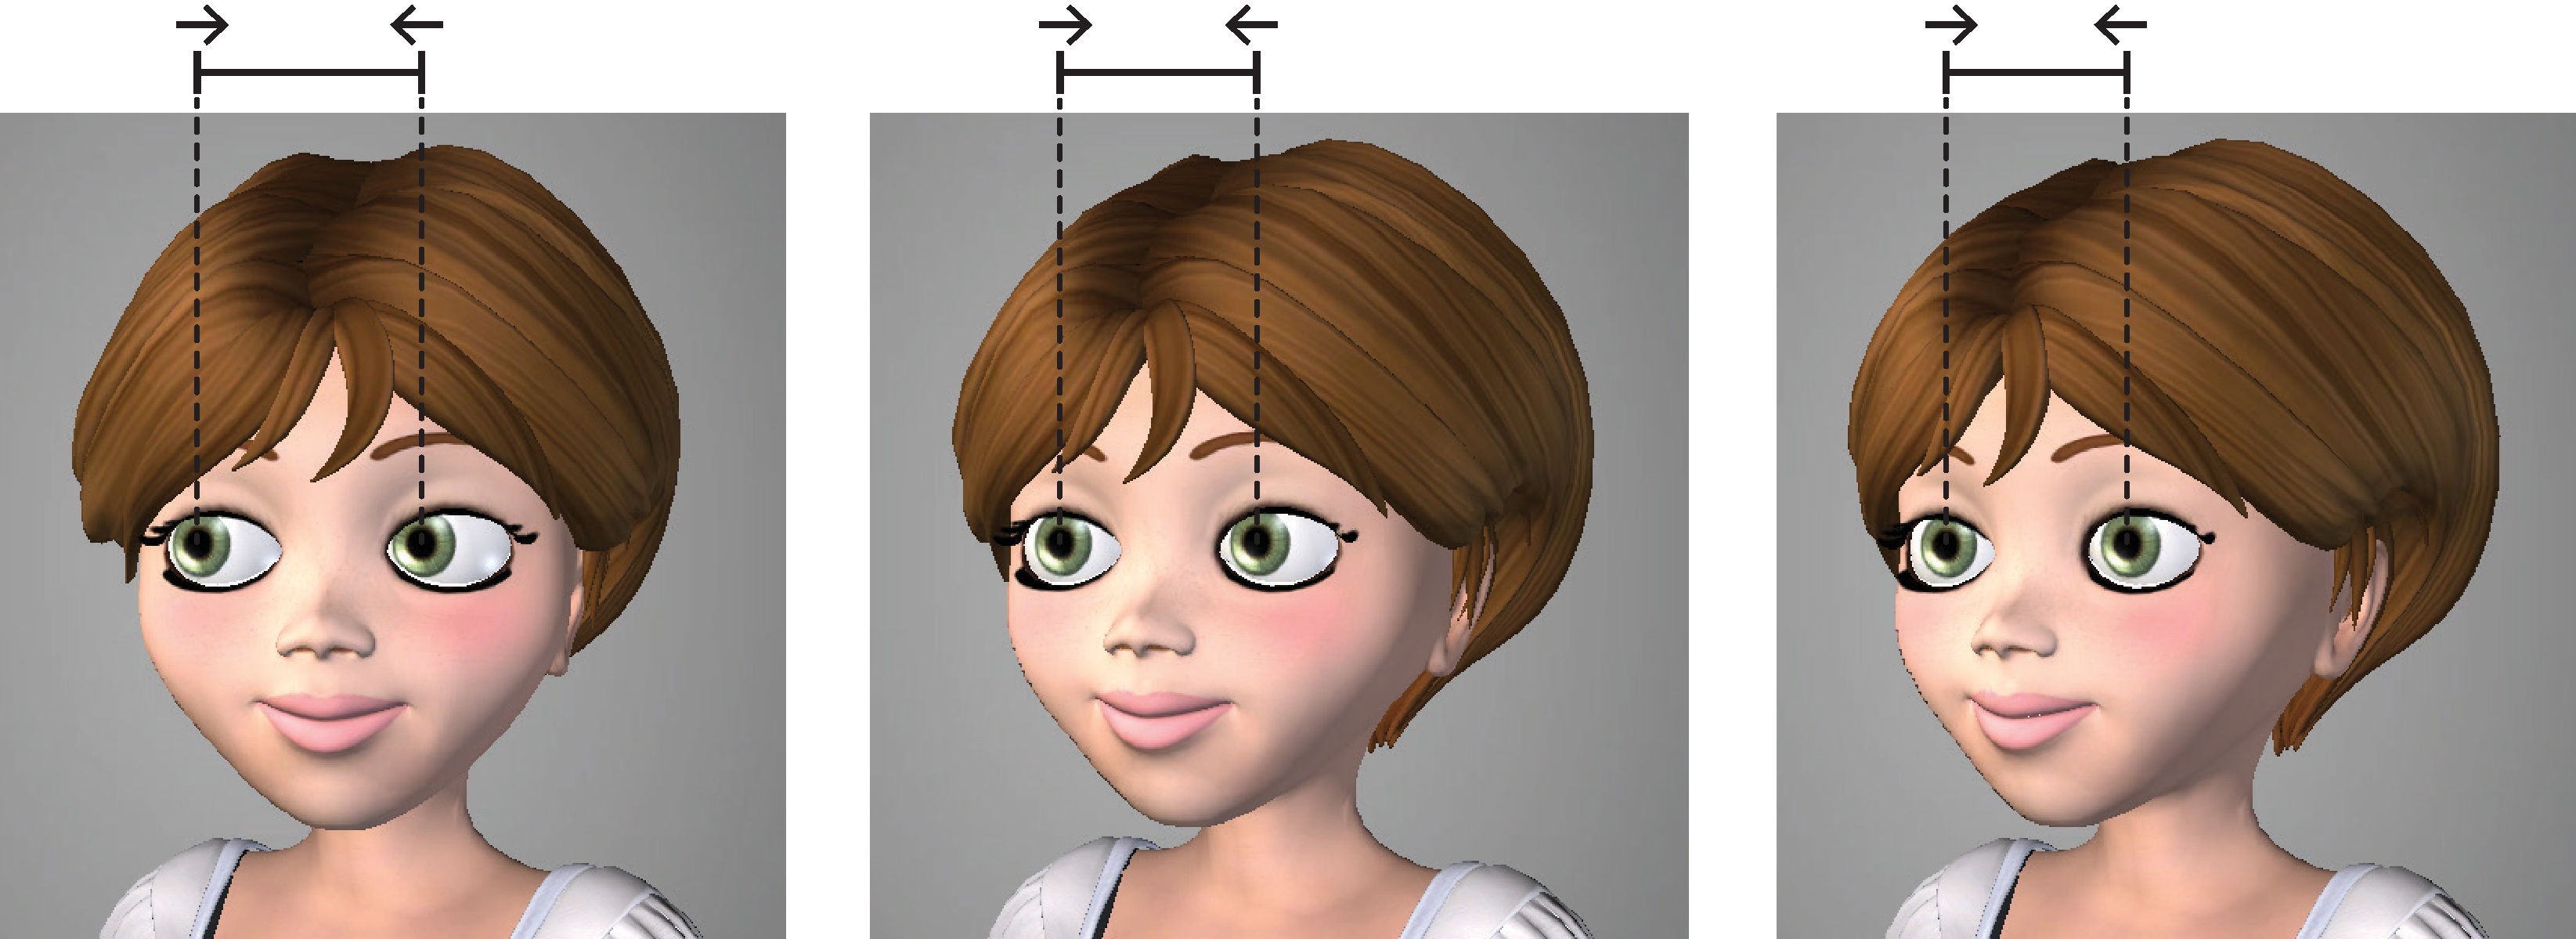
\includegraphics[width=0.48\textwidth]{Figures/EyeRetractionExample-small.pdf}
\caption{Eye retraction example. The right eye has aligned with the target and is retracting as the left eye moves forward. Notation: Solid line indicates inter-eye distance. Arrows $\rightarrow$ and $\leftarrow$ indicate eye movement direction.}
\vspace{-6pt}
\label{fig:EyeRetractionExample}
\end{figure}
% NOTE: Added better notation to all figures, and explanation in the caption of this one -- Tomislav

\begin{figure}[t]
\centering
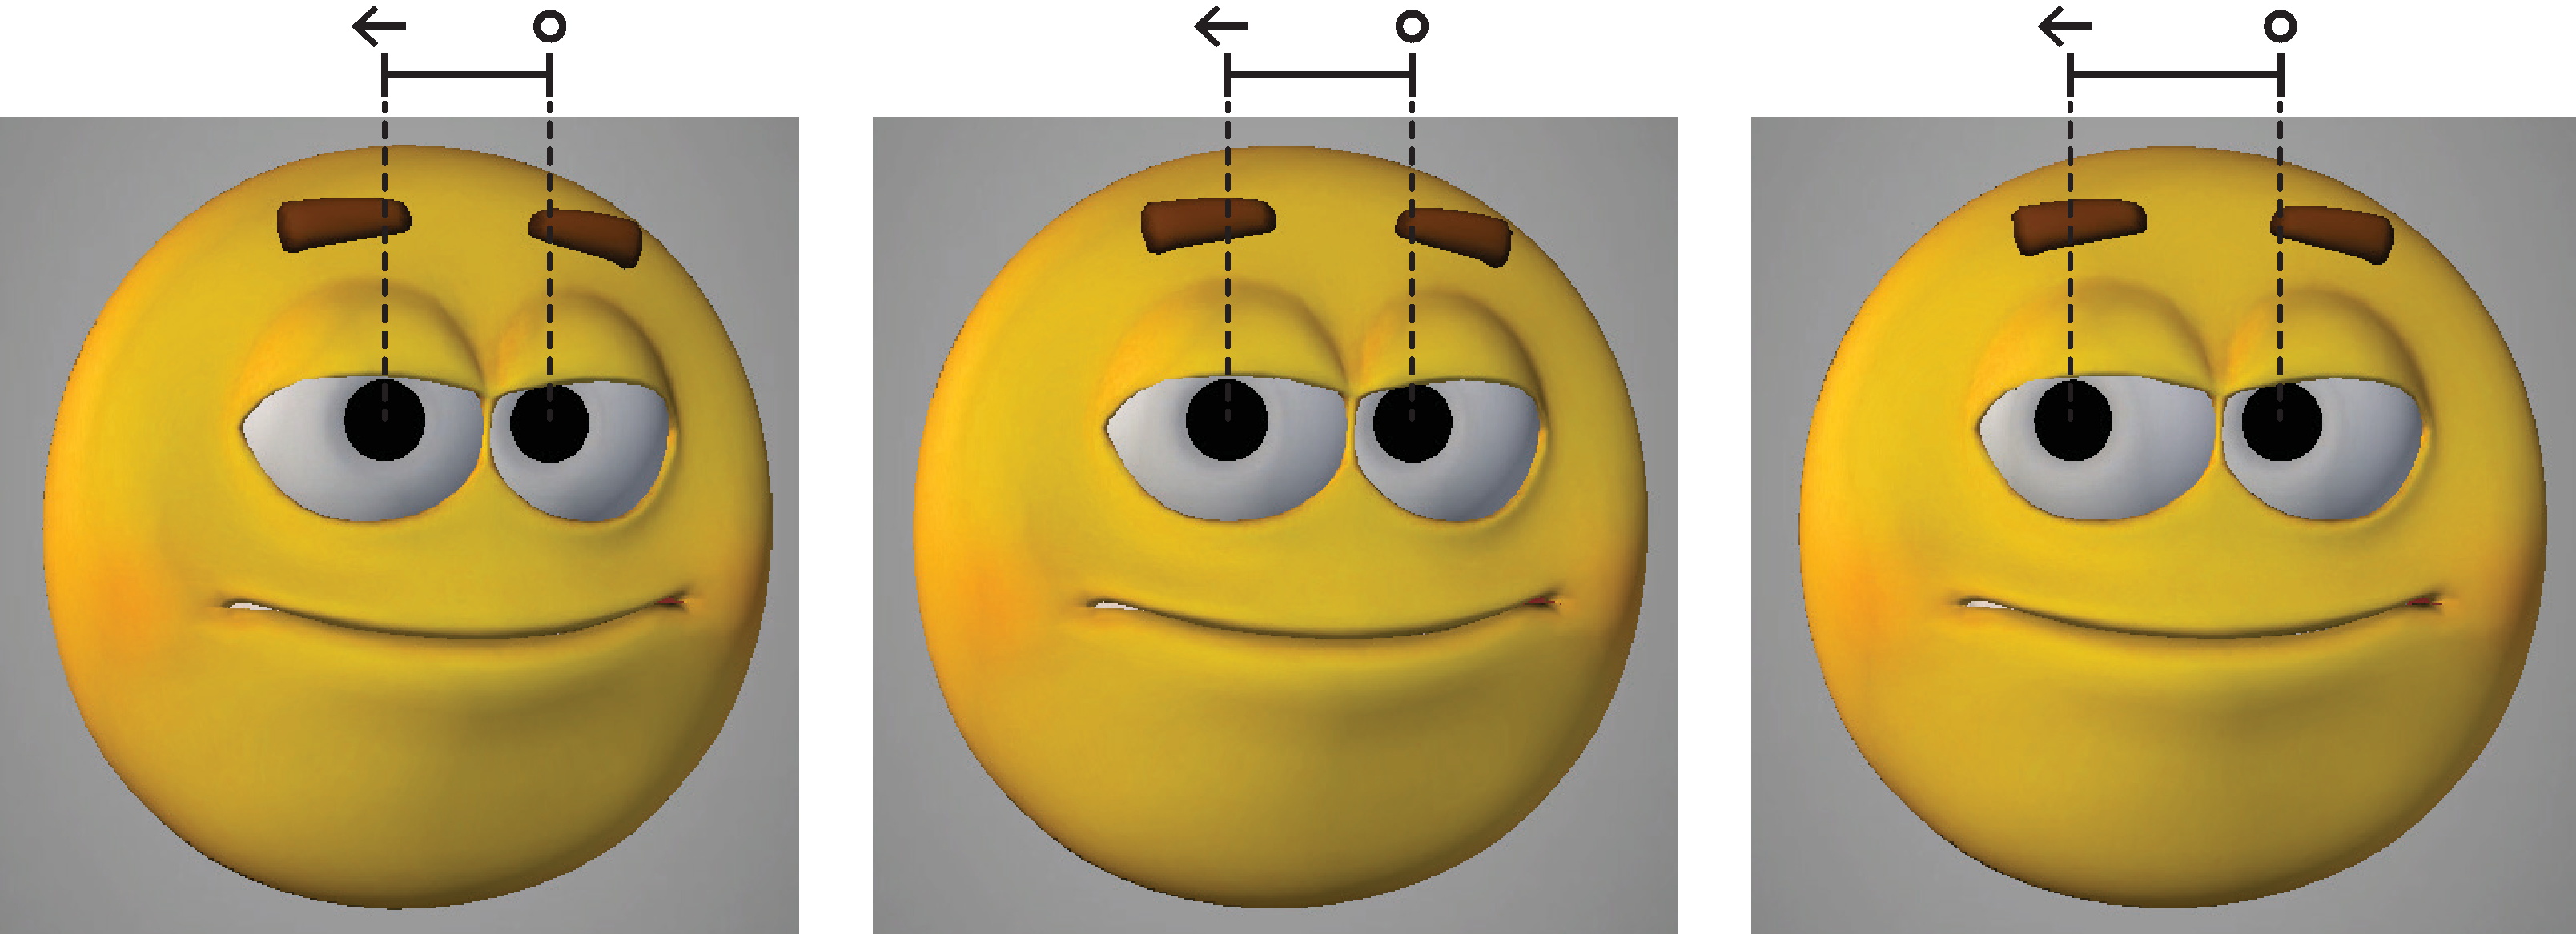
\includegraphics[width=0.48\textwidth]{Figures/StuckEyeExample-small.pdf}
\caption{Stuck eye example. The right eye is moving ahead, while the left eye is blocked by OMR. Notation: Dot $\circ$ indicates that the eye is stationary.}
\vspace{-10pt}
\label{fig:StuckEyeExample}
\end{figure}

\noindent\emph{Cross-eyedness} -- Cross-eyedness occurs when the eyes significantly angle inward (towards each other). In humans, while convergence on a target necessitate some amount of inward angle, excessive amounts are straining to maintain. Small amounts of cross-eyedness are not noticeable due to the small size of the eyes, and larger amounts are caused by unnatural viewing conditions or an explicit expression. In characters with large or widely spaced eyes, cross-eyedness becomes noticeable even in more standard viewing (Figure~\ref{fig:CrosseyednessFixExample}).

\noindent\emph{Speedy eyes} -- Human eyes have low mass and strong muscles that support fast and abrupt movements. In characters with larger eyes, such movements can appear implausible.

\noindent\emph{OMR-block} %(Figure~\ref{fig:OMRBlockExample})
--  When the eyes initiate a gaze shift and reach the boundary of the \textit{ocular motor range} (OMR), they are effectively blocked in their movements until the head brings them into alignment with the gaze target. While natural and common in humans, this phenomenon can appear anomalous in stylized characters; during this prolonged phase when the eyes are unable to move, the character may appear static and puppet-like. We believe this phenomenon to be caused by \textit{speedy eyes}; the eyes cover the distance between starting position and OMR in an unrealistic speed, resulting in an unusually long period of OMR-block. The visual artifact becomes even more prevalent with narrow OMR, a common property of stylized characters.

\noindent\emph{Eye retraction} -- In human gaze, when the head brings the eyes into alignment with the gaze target, the \textit{vestibulo-ocular reflex} (VOR) effectively locks the eyes onto the target as the head catches up, rotating the eyes in the opposite direction of the head movement. While this standard feature of human gaze does not appear as anomalous in real humans or characters with humanlike proportions, in stylized characters with large eyes, it can appear as if the eyes have overshot the target and are now suddenly retracting in order to realign with it (Figure~\ref{fig:EyeRetractionExample}). We believe that the cause of this illusion is excessive eye velocities that cause the eyes to advance further ahead and retract more than expected.

\noindent\emph{Stuck eye} -- Stuck eye is caused by asymmetry of eye shape, which necessarily involves asymmetry in the OMR. The leading eye in the gaze shift, which rotates outward, has a greater distance to cover before reaching OMR than the trailing eye. However, when both eyes move at the same velocity, as is the case with human eyes, the trailing eye will reach its OMR boundary sooner and become blocked, while the other eye will continue moving (Figure~\ref{fig:StuckEyeExample}). Movement in one eye does not occur in human gaze except in medical conditions such as amblyopia and therefore can appear abnormal.

\noindent\emph{Eye divergence} -- When the eyes have asymmetric OMR, their gaze directions can become divergent as they reach their respective OMR boundaries. Although difficult to observe in static poses, this divergence might cause disconjugate eye movements and appear jarring when the eyes are brought into alignment with the gaze target. In these movements, the leading eye will reach the gaze target before the trailing eye, and VOR causes the eye to rotate backward, while the trailing eye is still moving forward (Figure~\ref{fig:EyeDivergenceFixExample}). %This draws attention to the fact that eye orientations were divergent in the first place. 
Such divergent orientations and movements are improbable in healthy human gaze and appear anomalous.